\setcounter{section}{0}
\numberwithin{equation}{section}
\numberwithin{figure}{section}
\setcounter{chapter}{4}

\chapter{\texorpdfstring{The String $S$-matrix}{5 The string S-matrix}} \label{cha:5}

In Chapter 3, we expressed the $S$-matrix as a path integral over two-dimensional compact surfaces with vertex operators. In this chapter, we will reduce this path integral to a gauge-fixed form.

\section{The Circle and the Torus}\label{sec:5.1}

We identify a gauge slice, as shown in figure 3.7, as a choice of one configuration from each ($\text{diff} \times \text{Weyl}$) equivalence class. Locally, we achieve this by fixing the metric. However, globally, there exists a slight mismatch between the space of metrics and the worldsheet gauge group.

Once again, the point particle serves as an excellent illustration. We wish to calculate the Euclidean path integral:
\begin{equation}
	\int[d e d X] \exp \left[-\frac{1}{2} \int d \tau\left(e^{-1} \dot{X}^{\mu} \dot{X}_{\mu}+e m^{2}\right)\right]
\end{equation}
Consider paths that form closed loops in spacetime, so the topology is a circle. The parameter $\tau$ takes values between 0 and 1, where the endpoints are equivalent. That is, $X^{\mu}(\tau)$ and $e(\tau)$ are periodic on $0 \leq \tau \leq 1$. The einbein $e(\tau)$ has one component, and there exists a local symmetry that completely determines the einbein.

The einbein transforms as $e^{\prime} d \tau^{\prime}=e d \tau$, so the gauge choice yields a differential equation for $\tau^{\prime}(\tau)$:
\begin{equation}
	\frac{\partial \tau^{\prime}}{\partial \tau}=e(\tau)
\end{equation}
Integrating this with the boundary condition $\tau^{\prime}(0)=0$ determines:
\begin{equation}
	\tau^{\prime}(\tau)=\int_{0}^{\tau} d \tau^{\prime \prime} e\left(\tau^{\prime \prime}\right)
\end{equation}
The problem is that, in general, $\tau^{\prime}(1) \neq 1$, so periodicity is not preserved. In fact,
\begin{equation}
	\tau^{\prime}(1)=\int_{0}^{1} d \tau e(\tau)=l
\end{equation}
is the invariant length of the circle. Therefore, we cannot set $e^{\prime}=1$ while keeping the coordinate range invariant. We can either keep the coordinate range fixed and let $e^{\prime}$ be a constant value $e^{\prime}=l$, or let $e^{\prime}=1$ and allow the coordinate range to vary:
\begin{subequations}
	\begin{equation}
		e^{\prime}=l, \quad 0 \leq \tau \leq 1
	\end{equation}
	or
	\begin{equation}
		e^{\prime}=1, \quad 0 \leq \tau \leq l
	\end{equation}\label{5.1.5}
\end{subequations}
In either case, after fixing the gauge invariance, we are left with a universal integral over $l$.

In other words, not all einbeins on a circle are equivalent. There exists a single-parameter family of inequivalent einbeins, parameterized by $l$. The two descriptions in (5.1.5) both have analogs in string theory. Actually, we will use a description similar to (5.1.5a) to define the path integral, where the fields are functions on a fixed coordinate range, and then transform to a description like (5.1.5b), where the metric is fixed and the moduli are encoded within the coordinate range.

There is a second difficulty related to gauge fixing. The condition $e = \text{constant}$ is preserved by rigid translations:
\begin{equation}
	\tau \rightarrow \tau+v \bmod 1
\end{equation}
That is, on a circle, we cannot say where the origin is. Consequently, fixing the metric leaves a small portion of unfixed local symmetry, resulting in a mismatch in both directions. The metric is not equivalent to another gauge, and the gauge transformation is not fixed by the choice of metric.

Moving to strings, we take the torus as an example, where the same difficulties arise. Starting from the coordinate region:
\begin{equation}
	0 \leq \sigma^{1} \leq 2 \pi, \quad 0 \leq \sigma^{2} \leq 2 \pi
\end{equation}
where $X^{\mu}\left(\sigma^{1}, \sigma^{2}\right)$ and $g_{a b}\left(\sigma_{1}, \sigma_{2}\right)$ are periodic in both directions. Equivalently, we can view this as point equivalence on the $\sigma$ plane:
\begin{equation}
	\left(\sigma^{1}, \sigma^{2}\right) \cong\left(\sigma^{1}, \sigma^{2}\right)+2 \pi(m, n)\label{5.1.8}
\end{equation}
where $m, n$ are integers.

To what extent is the field space $\text{diff} \times \text{Weyl}$ redundant? The theorem is that it is impossible to transform a general metric into a unit form through a $\text{diff} \times \text{Weyl}$ transformation that keeps the periodicity (5.1.7) invariant, but it can be transformed into:
\begin{equation}
	d s^{2}=\left|d \sigma^{1}+\tau d \sigma^{2}\right|^{2};\qquad g_{ab}=\begin{bmatrix}
		1 & \Re{\tau}\\
		\Re{\tau} & |\tau|^2
	\end{bmatrix}\label{5.1.9}
\end{equation}
where $\tau$ is a complex constant. When $\tau=i$, this is the unit metric $\delta_{a b}$.

To see this, we repeat the steps used in the local discussion of section \ref{sec:3.3}. First, we can make the metric flat through a Weyl transformation satisfying $2 \nabla^{2} \omega=R$. By expanding the eigenmodes of $\nabla^{2}$, it can be seen that under periodic boundary conditions, there is a unique solution for $\omega$ up to an additive constant. What is important here is $\int d^{2} \sigma g^{1 / 2} R$, which is $4 \pi$ times the Euler number, and for a torus, this is zero. Afterwards, a transformation to new coordinates $\tilde{\sigma}^{a}$ turns the metric into unit form. However, just as in the point particle case, there is no guarantee that this reflects the original periodicity. Instead, we may now have:
\begin{equation}
	\tilde{\sigma}^{a} \cong \tilde{\sigma}^{a}+2 \pi\left(m u^{a}+n v^{a}\right)
\end{equation}
where $u^{a}, v^{a}$ are general translations. By rotating and scaling the coordinate system, accompanied by an $\omega$ shift that keeps the metric normalized, we can always set $u=(1,0)$. This leaves two parameters, the components of $v$.

Defining $w=\tilde{\sigma}^{1}+i \tilde{\sigma}^{2}$, the metric is $d w d \bar{w}$ and the periodicity is:
\begin{equation}
	w \cong w+2 \pi(m+n \tau)\label{5.1.11}
\end{equation}
where $\tau=v^{1}+i v^{2}$. The torus is a parallelogram with periodic boundary conditions in the $w$ plane, as shown in figure (\ref{Fig5.1}).

\begin{figure}[!htbp]
	\begin{center}
		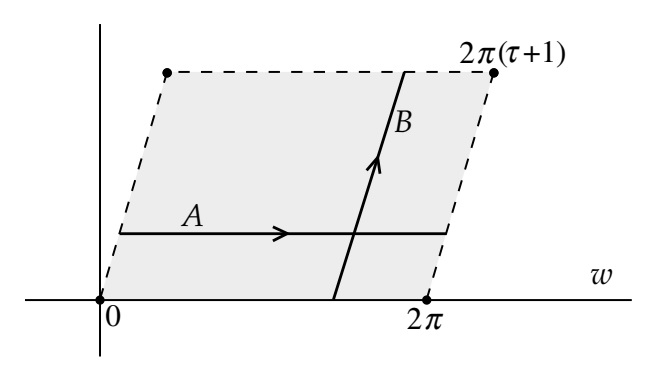
\includegraphics[width=0.5\textwidth]{figure/Fig5.1.jpg}\\
		\caption{Torus with modulus $\tau$, in gauge $d s^{2}=d w d \bar{w}$. The upper and lower edges are identified, as are the right- and left-hand edges. Closed curves $A$ and $B$ are marked for later reference.}\label{Fig5.1}
	\end{center}
\end{figure}

Alternatively, using $\sigma^{a}$, $w=\sigma^{1}+\tau \sigma^{2}$ is defined. The original periodicity is preserved, but the metric takes the more general form \eqref{5.1.9}. The integration over the metric reduces to two integrals over the real and imaginary parts of $\tau$. The metric \eqref{5.1.9} is invariant under complex conjugation and degenerates for real $\tau$, so we can focus our attention on $\operatorname{Im} \tau > 0$. Just as in the circular case \eqref{5.1.5}, we can put these parameters into the metric \eqref{5.1.9} or the periodicity \eqref{5.1.11}. The parameter $\tau$ is called the Teichmüller parameter or, more generally, the modulus.

Unlike the point particle, there is no simple invariant expression for $\tau$ analogous to the invariant length of a circle. There is some additional redundancy that has no analog in the point particle case. The value $\tau+1$ generates the same equivalence set (5.1.11) as $\tau$, replacing $(m, n) \rightarrow(m-n, n)$. The same is true for $-1 / \tau$. Defining $w^{\prime}=\tau w$ and replacing $(m, n) \rightarrow(n,-m)$, repeatedly using these two transformations:
\begin{equation}
	T: \quad \tau^{\prime}=\tau+1, \quad S: \tau^{\prime}=-1 / \tau
\end{equation}
generates:
\begin{equation}
	\tau^{\prime}=\frac{a \tau+b}{c \tau+d}\label{5.1.13}
\end{equation}
where $a, b, c, d$ are integers satisfying $a d-b c=1$.

We can also consider it as follows: the transformation
\begin{equation}
	\left[\begin{array}{l}
		\sigma^{1} \\
		\sigma^{2}
	\end{array}\right]=\left[\begin{array}{ll}
		d & b \\
		c & a
	\end{array}\right]\left[\begin{array}{l}
		\sigma^{\prime 1} \\
		\sigma^{\prime 2}
	\end{array}\right]\label{5.1.14}
\end{equation}
turns the $\sigma$ metric \eqref{5.1.9} into the same form of metric in $\sigma^{\prime}$ but with modulus $\tau^{\prime}$. This is a diffeomorphism mapping of the torus. Since $a d-b c=1$, it is a one-to-one mapping and preserves the periodicity \eqref{5.1.8}. However, it cannot be obtained from a continuous infinitesimal transformation starting from the identity---it is a so-called large coordinate transformation. Curve $A$ in coordinates $\sigma$ maps to a curve in $\sigma^{\prime}$ stretched $a$ times along the $A^{\prime}$ direction and $c$ times along the $B^{\prime}$ direction.

These large coordinate transformations form the group $SL(2, \mathbf{Z})$. The group on the $\tau$ plane is $SL(2, \mathbf{Z}) / \mathbf{Z}_{2} = PSL(2, \mathbf{Z})$, because if the signs of $a, b, c, d$ are all flipped, $\tau^{\prime}$ remains invariant. The group of transformations \eqref{5.1.14} is called the modular group. Using the modular transformation \eqref{5.1.13}, it can be proved that every $\tau$ is equivalent to a point in the region $F_{0}$, as shown in figure (\ref{Fig5.2}).

\begin{figure}[!htbp]
	\begin{center}
		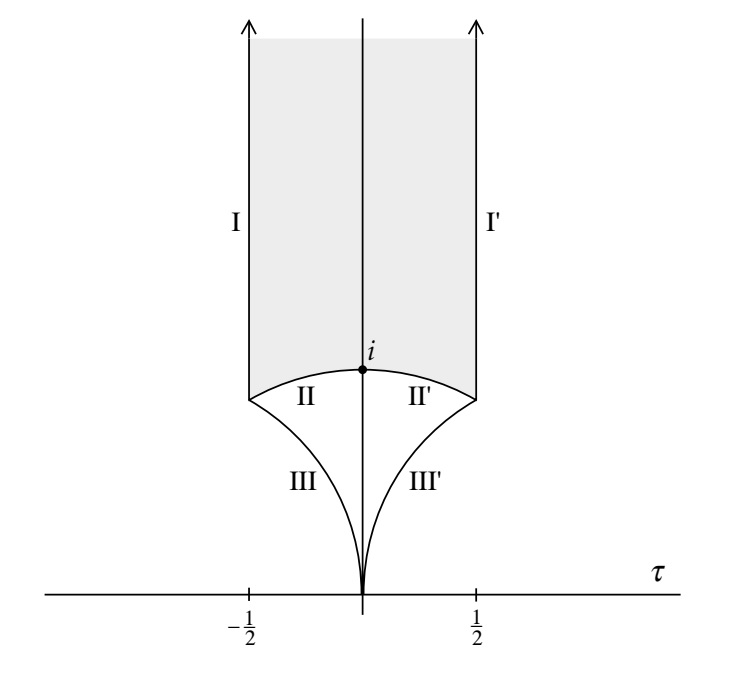
\includegraphics[width=0.5\textwidth]{figure/Fig5.2.jpg}\\
		\caption{The standard fundamental region $F_{0}$ for the moduli space of the torus, shaded. The lines I and I' are identified, as are the arcs II and II'. A different fundamental region, mapped into $F_{0}$ by the modular transformation $S$, is bounded by II, II', III, and III'.}\label{Fig5.2}
	\end{center}
\end{figure}

\begin{equation}
	-\frac{1}{2} \leq \operatorname{Re} \tau \leq \frac{1}{2}, \quad|\tau| \geq 1
\end{equation}
Except for the boundaries identified in the figure, this is called the fundamental region of the upper half-plane modulo $PSL(2, \mathbf{Z})$. Due to the equivalence, $F_{0}$ can be considered rolled up, opening only when $\operatorname{Im} \tau \rightarrow \infty$. The fundamental region $F_{0}$ is a representation of the moduli space of ($\text{diff} \times \text{Weyl}$) inequivalent metrics.

There are further difficulties, as with the point particle. Requiring the metric to take the form (5.1.9) where $\tau$ is in a given fundamental region does not fix all $\text{diff} \times \text{Weyl}$ invariance. The metric and periodicity are invariant under rigid translations:
\begin{equation}
	\sigma^{a} \rightarrow \sigma^{a}+v^{a}
\end{equation}
So this two-parameter $\text{diff} \times \text{Weyl}$ subgroup is not fixed. Additionally, the discrete transformation $\sigma^{a} \rightarrow-\sigma^{a}$ leaves the metric invariant, and in the non-oriented case, $\tau \rightarrow-\bar{\tau}$ via $\left(\sigma^{1}, \sigma^{2}\right) \rightarrow\left(-\sigma^{1}, \sigma^{2}\right)$ also leaves the metric invariant. Thus, there is again a mismatch between metric degrees of freedom and local symmetries: parameters in the metric cannot be removed by symmetry, and symmetry is not fixed by the choice of metric. Unfixed symmetries are called the Conformal Killing Group (CKG).

When there are enough vertex operators in the amplitude, we can completely fix the gauge invariance by fixing the positions of certain vertex operators. On a torus with $n$ vertex operators, the invariance (5.1.16) can be used to fix the position of one vertex operator, leaving the integral over $\tau$ and $n-1$ other positions. The $\mathbf{Z}_{2}$ from $\sigma^{a} \rightarrow-\sigma^{a}$ can be used to fix a second vertex operator in the middle of the torus. In practice, for finite redundancy counts, it is often more convenient to leave some symmetries unfixed and divide by a suitable factor. Additionally, if there are too few vertex operators and some Conformal Killing invariance remains unfixed, then we must explicitly account for the redundancy count.

\subsubsection*{\Large Note to the Reader}
In the remainder of this chapter, we will discuss moduli more generally. The primary goal is the gauge-fixed expression for the string $S$-matrix \eqref{5.3.9}. In fact, most interesting string physics can be seen in tree-level and one-loop amplitudes. For this reason, the measure can be obtained through shortcuts. For tree amplitudes, there are no metric moduli but the positions of certain vertex operators must be fixed. The measure can be reasoned out as explained below \eqref{6.4.4}. For one-loop amplitudes, the measure can be understood in a relatively intuitive way by analogy with the discussion of point particles below \eqref{7.3.9}.

\section{Moduli and Riemann Surfaces}\label{sec:5.2}

Now, we repeat the above discussion in a more general and abstract way. We integrate over all metrics on some given topology $r$. Call this metric space $\mathscr{G}_{r}$. For closed oriented surfaces, we can label $r$ by the number of handles $g$, also called the genus. After accounting for $\text{diff} \times \text{Weyl}$ redundancy, we are left with the moduli space:
\begin{equation}
	\mathscr{M}_{r}=\frac{\mathscr{G}_{r}}{(\text { diff } \times \mathrm{Weyl})_{r}}
\end{equation}
Just as in the torus case, this space is parameterized by a finite number of moduli. For the torus, $\mathscr{M}_{1}$ is the upper half-plane modulo $PSL(2, \mathbf{Z})$, or equivalently any fundamental region such as $F_{0}$. There may also exist a $\text{diff} \times \text{Weyl}$ subgroup, the CKG, that leaves the metric invariant.

When vertex operators are present in the path integral, it is useful to treat their positions on an equal footing with the moduli in the metric. When we need to make a distinction, we will refer to metric moduli. One way to handle the CKG, which is applicable if vertex operators exist in the path integral, is to further specify the gauge by fixing the positions of certain vertex operators. The Polyakov path integral includes an integration over $\mathscr{G}_{r}$ and an integration of $n$ vertex operators over the worldsheet $\mathscr{M}$. The moduli space with vertex operators on topology $r$ is:
\begin{equation}
	\mathscr{M}_{r, n}=\frac{\mathscr{G}_{r} \times M^{n}}{(\text { diff } \times \mathrm{Weyl})_{r}}
\end{equation}
As we saw for the torus, $\operatorname{diff}_{r}$ is generally not connected. Selecting the connected component $\text{diff}_{r 0}$ containing the identity, the quotient
\begin{equation}
	\frac{\operatorname{diff}_{r}}{\operatorname{diff}_{r 0}}
\end{equation}
is the modular group.

It is interesting to study the $\text{diff} \times \text{Weyl}$ redundancy of the metric at the infinitesimal level. That is, searching for metric variations that are not equivalent to a $\text{diff} \times \text{Weyl}$ transformation and are thus equivalent to a change in moduli. We also want to find certain $\text{diff} \times \text{Weyl}$ transformations that do not change the metric; these are the infinitesimal elements of the CKG, called Conformal Killing Vectors (CKVs).

An infinitesimal $\text{diff} \times \text{Weyl}$ transformation changes the metric by:
\begin{equation}
	\delta g_{a b}=-2\left(P_{1} \delta \sigma\right)_{a b}+(2 \delta \omega-\nabla \cdot \delta \sigma) g_{a b}\label{5.2.4}
\end{equation}
where $P_{1}$ is the traceless symmetric linear combination of derivatives (3.3.17). The metric variation $\delta^{\prime} g_{a b}$ corresponding to the moduli is orthogonal to all variations (5.2.4):
\begin{equation}
	\begin{aligned}
		0 &=\int d^{2} \sigma g^{1 / 2} \delta^{\prime} g_{a b}\left[-2\left(P_{1} \delta \sigma\right)^{a b}+(2 \delta \omega-\nabla \cdot \delta \sigma) g^{a b}\right] \\
		&=\int d^{2} \sigma g^{1 / 2}\left[-2\left(P_{1}^{T} \delta^{\prime} g\right)_{a} \delta \sigma^{a}+\delta^{\prime} g_{a b} g^{a b}(2 \delta \omega-\nabla \cdot \delta \sigma)\right]
	\end{aligned}\label{5.2.5}
\end{equation}
where the adjoint is $\left(P_{1}^{T} u\right)_{a}=-\nabla^{b} u_{a b}$.

\begin{tcolorbox}[breakable]
	Note:
	\begin{align*}
		(P_1\delta \sigma)^{a b}&=\frac{1}{2}\left(\nabla^{a} \delta \sigma^{b}+\nabla^{b} \delta \sigma^{a}-g^{a b} \nabla \cdot \delta \sigma\right) \\
		\delta^{\prime} g_{a b}(P_1 \delta \sigma)^{a b}&=\frac{1}{2}\left(\delta^{\prime} g_{a b} \nabla^{a} \delta \sigma^{b}+\delta^{\prime} g_{a b} \nabla^{b} \delta \sigma^{a}-\delta^{\prime} g_{a b} g^{a b} \nabla \cdot \delta \sigma\right)
	\end{align*}
\end{tcolorbox}

In order to make the overlap \eqref{5.2.5} zero for general $\delta \omega$ and $\delta \sigma$, we require
\begin{subequations}
	\begin{equation}
		g^{a b} \delta^{\prime} g_{a b} =0 
	\end{equation}	
	\begin{equation}
		\left(P_{1}^{T} \delta^{\prime} g\right)_{a} =0
	\end{equation}			\label{5.2.6}
\end{subequations}
The first condition requires $\delta^{\prime} g_{a b}$ to be traceless, and it is a traceless symmetric tensor in the kernel of $P_{1}^{T}$. For each solution to these equations, there exists a modulus.

CKVs are those $\delta \sigma$ such that $\delta g_{a b}=0$ in \eqref{5.2.4}. The trace of this equation uniquely determines $\delta \omega$, leaving the Conformal Killing Equation:
\begin{equation}
	\left(P_{1} \delta \sigma\right)_{a b}=0\label{5.2.7}
\end{equation}
Equations \eqref{5.2.6} and (\ref{5.2.7}) become simple for variations around the conformal gauge:
\begin{subequations}
	\begin{equation}
		\partial_{\bar{z}} \delta^{\prime} g_{z z} =\partial_{z} \delta^{\prime} g_{\bar{z} \bar{z}}=0 
	\end{equation}	
	\begin{equation}
		\partial_{\bar{z}} \delta z =\partial_{z} \delta \bar{z}=0
	\end{equation}			\label{5.2.8}
\end{subequations}
Thus, the variation of the moduli corresponds to holomorphic quadratic differentials, and CKVs correspond to holomorphic vector fields. On a torus, the only holomorphic bi-periodic functions are constants, so there are two real moduli and two real CKVs, consistent with the previous section's discussion.

The metric moduli correspond to the kernel of $P_{1}^{T}$ \eqref{5.2.6}, while CKVs correspond to the kernel of $P_{1}$ \eqref{5.2.7}. The Riemann-Roch theorem relates the number of metric moduli $\mu=\operatorname{dim} \operatorname{ker} P_{1}^{T}$ and the number of CKVs $\kappa=\operatorname{dim} \operatorname{ker} P_{1}$ to the Euler number $\chi$:
\begin{equation}
	\mu-\kappa=-3 \chi\label{5.2.9}
\end{equation}
We will derive it later in this chapter. For closed oriented surfaces, $-3 \chi=6 g-6$. This count is for real moduli, splitting complex moduli like $\tau$ into real and imaginary parts.

Furthermore, $\kappa$ is zero for $\chi < 0$, and $\mu$ is zero for $\chi > 0$. To prove this, we cite the following property: one can always find a metric via Weyl transformation such that the scalar curvature $R$ is constant. In this case, $R$ has the same sign as $\chi$. Now, $P_{1}^{T} P_{1}=-\frac{1}{2} \nabla^{2}-\frac{1}{4} R$, so
\begin{equation}
	\begin{aligned}
		\int d^{2} \sigma g^{1 / 2}\left(P_{1} \delta \sigma\right)_{a b}\left(P_{1} \delta \sigma\right)^{a b} &=\int d^{2} \sigma g^{1 / 2} \delta \sigma_{a}\left(P_{1}^{T} P_{1} \delta \sigma\right)^{a} \\
		&=\int d^{2} \sigma g^{1 / 2}\left(\frac{1}{2} \nabla_{a} \delta \sigma_{b} \nabla^{a} \delta \sigma^{b}-\frac{R}{4} \delta \sigma_{a} \delta \sigma^{a}\right)
	\end{aligned}\label{5.2.10}
\end{equation}
For negative $\chi$, the right side is strictly positive definite, so $P_{1} \delta \sigma$ cannot be zero. A similar argument shows that for positive $\chi$, $P_{1}^{T} \delta^{\prime} g$ cannot be zero. Combining these results, we have:
\begin{subequations}
	\begin{equation}
		\chi>0:  \kappa=3 \chi, \quad \mu=0 
	\end{equation}
	\begin{equation}
		\chi<0:  \kappa=0, \quad \mu=-3 \chi
	\end{equation}				\label{5.2.11}		
\end{subequations}

\subsubsection*{\Large Riemann Surfaces}
A common way to describe the moduli space is to choose a metric from each equivalence class, which forms a family of metrics $\hat{g}_{a b}(t ; \sigma)$ depending on moduli $t^{k}$. For the torus, \eqref{5.1.9} gives such a slice. Using the other description \eqref{5.1.11} is often more convenient, where $d w d \bar{w}$ is fixed and the moduli are encoded in the coordinate range. We can formalize this concept as follows.

Recall how a differentiable manifold is defined. A manifold is covered by a set of overlapping charts, where $\sigma_{m}^{a}$ are the coordinates in the $m$-th coordinate chart. When charts $m$ and $n$ overlap, the coordinates in the two charts are related by:
\begin{equation}
	\sigma_{m}^{a}=f_{m n}^{a}\left(\sigma_{n}\right) \label{5.2.12}		
\end{equation}
where transition functions are required to be differentiable. For a Riemannian manifold, each chart is also given a metric $g_{m, a b}\left(\sigma_{m}\right)$, and the values in the overlap region are related by the usual tensor laws.

For a complex manifold, each chart has complex coordinates $z_{m}^{a}$. Transition functions are required to be holomorphic:
\begin{equation}
	z_{m}^{a}=f_{m n}^{a}\left(z_{n}\right)\label{5.2.13}		
\end{equation}
Since holomorphicity does not depend on the coordinates $z_{m}^{a}$ used. Holomorphic functions on the manifold can now be defined. Just as two differentiable manifolds are equivalent if there exists a one-to-one differentiable mapping between them, two complex manifolds are equivalent if there exists a one-to-one holomorphic mapping between them.

In the two-dimensional case (one complex coordinate), the complex manifold is called a Riemann surface. In this case, there is a one-to-one correspondence:
\begin{equation}
	\text{Riemann surfaces} \leftrightarrow \text{Riemannian manifolds mod Weyl}
\end{equation}
We place 'mod Weyl' on the right because 'mod diff' is already implied in the definition of a Riemannian manifold. To see this isomorphism, start from the Riemannian manifold. From our discussion of conformal gauge, we know we can find $z_{m}$ in each chart such that:
\begin{equation}
	d s^{2} \propto d z_{m} d \bar{z}_{m}
\end{equation}
In adjacent charts, coordinates need not be identical, but since $d s^{2} \propto d z_{m} d \bar{z}_{m} \propto d z_{n} d \bar{z}_{n}$, the transition functions are holomorphic. This is a mapping from Riemannian manifolds to two-real-dimensional complex manifolds. For the inverse mapping, one can take metric $d z_{m} d \bar{z}_{m}$ in the $m$-th chart and smooth it in the overlap region to produce a Riemannian manifold. The two characterizations of Riemann surfaces are thus equivalent.

The description of the torus using the complex coordinate $w$ of the parallelogram (\ref{Fig5.1}) illustrates the idea of a complex manifold. Imagine taking a single coordinate chart slightly larger than the basic parallelogram of (\ref{Fig5.1}). The periodicity conditions
\begin{equation}
	w \cong w+2 \pi \cong w+2 \pi \tau
\end{equation}
are the transition functions on the overlap of the two opposite edges of the coordinate chart. These transition functions define the surface. To define the original path integral over the metric, treating the metric as fixed coordinates, such as the square (5.1.7), or at least a fixed set of coordinate charts with fixed transition functions, is the simplest starting point. To study quantum field theory on a given surface, the simplest approach is to handle unit metrics where transition function moduli are related, as in the parallelogram (5.1.11).

One can also see Riemann surfaces as follows. Define the worldsheet as a union of coordinate charts. We can use $\text{diff} \times \text{Weyl}$ degrees of freedom to reach the metric $d z d \bar{z}$ in each chart. Then the gauge choices in the chart overlap can only differ by the $\text{diff} \times \text{Weyl}$ invariance of this metric. This is exactly the conformal transformation we discussed. Thus, Riemann surfaces are the natural place for CFT to grow, because fields in CFT have clear transformation properties under conformal transformations.

\section{The Measure for Moduli}\label{sec:5.3}
We now review the gauge fixing of the Polyakov path integral. We already know that gauge redundancy does not completely eliminate the path integral over the metric, but leaves a finite-dimensional integral over the moduli space. To account for this, it is necessary to refine the discussion of section 3.3.

The path integral for the $S$-matrix is:
\begin{equation}
	\begin{aligned}
		&S_{j_{1} \ldots j_{n}}\left(k_{1}, \ldots, k_{n}\right) \\
		&\quad=\sum_{\text { topologies }} \int \frac{[d \phi d g]}{V_{\text {diff } \times \text { Weyl }}} \exp \left(-S_{\mathrm{m}}-\lambda \chi\right) \prod_{i=1}^{n} \int d^{2} \sigma_{i} g\left(\sigma_{i}\right)^{1 / 2} \mathscr{V}_{j_{i}}\left(k_{i}, \sigma_{i}\right)
	\end{aligned}\label{5.3.1}
\end{equation}
This is the previous expression \eqref{3.5.5}, but now with a universal matter field $c=\tilde{c}=26$, where matter fields are labeled by $\phi$. In gauge fixing, the integration over the metric and positions is replaced by an integration over the gauge group, moduli, and unfixed positions:
\begin{equation}
	[d g] d^{2 n} \sigma \rightarrow[d \zeta] d^{\mu} t d^{2 n-\kappa} \sigma\label{5.3.2}
\end{equation}
After factoring out the gauge volume, the Jacobian of this transformation becomes the measure on the moduli space.

This step is identical to section \ref{sec:3.3}, now accounting for moduli and CKVs. Specifically, the gauge choice now fixes $\kappa$ vertex coordinates, $\sigma_{i}^{a} \rightarrow \hat{\sigma}_{i}^{a}$. Denoting the set of fixed coordinates $(a, i)$ as $f$, define the Faddeev-Popov measure on the moduli space as:
\begin{equation}
	1=\Delta_{\mathrm{FP}}(g, \sigma) \int_{F} d^{\mu} t \int_{\mathrm{diff} \times \mathrm{Weyl}}[d \zeta] \delta\left(g-\hat{g}(t)^{\zeta}\right) \prod_{(a, i) \in f} \delta\left(\sigma_{i}^{a}-\hat{\sigma}_{i}^{\zeta a}\right)\label{5.3.3}
\end{equation}
By definition, each metric $(\text{diff} \times \text{Weyl})$ is equivalent to a $\hat{g}(t)$ for some $t$ and $\zeta$. In fact, as discussed at the end of section \ref{sec:5.1}, there might be a residual discrete symmetry group of finite order $n_{R}$, so the delta function is non-zero at $n_{R}$ points.

Substituting \eqref{5.3.3} into the path integral \eqref{5.3.1} and using the same steps as before gives:
\begin{equation}
	\begin{aligned}
		S_{j_{1} \ldots j_{n}}\left(k_{1}, \ldots, k_{n}\right)=& \sum_{\text {topologies}} \int_{F} d^{\mu} t \Delta_{\mathrm{FP}}(\hat{g}(t), \hat{\sigma}) \int[d \phi] \int \prod_{(a, i) \notin f} d \sigma_{i}^{a} \\	
		&\times \exp \left(-S_{\mathrm{m}}[\phi, \hat{g}(t)]-\lambda \chi\right) \prod_{i=1}^{n}\left[\hat{g}\left(\sigma_{i}\right)^{1 / 2} \mathscr{N}_{j_{i}}\left(k_{i} ; \sigma_{i}\right)\right]
	\end{aligned}\label{5.3.4}
\end{equation}
The integration over metrics and vertex operator coordinates now reduces to an integration over the moduli space $F$ plus unfixed coordinates with the measure given by $\Delta_{\mathrm{FP}}$. In the vertex operators, $\kappa$ positions are fixed.

Now we calculate the Faddeev-Popov measure. The delta function is non-zero at $n_R$ points related by symmetry, so we consider one such point and divide by $n_R$. Expand the definition of $\Delta_{\mathrm{FP}}$ in \eqref{5.3.3} near this point. A general metric variation equals a local symmetry variation plus a change in moduli $t^k$:
\begin{equation}
	\delta g_{a b}=\sum_{k=1}^{\mu} \delta t^{k} \partial_{t^{k}} \hat{g}_{a b}-2\left(\hat{P}_{1} \delta \sigma\right)_{a b}+(2 \delta \omega-\hat{\nabla} \cdot \delta \sigma) \hat{g}_{a b}\label{5.3.5}
\end{equation}
The Faddeev-Popov inverse determinant is:
\begin{equation}
	\begin{aligned}
		\Delta_{\mathrm{FP}}(\hat{g}, \hat{\sigma})^{-1} &=n_{R} \int d^{\mu} \delta t[d \delta \omega d \delta \sigma] \delta\left(\delta g_{a b}\right) \prod_{(a, i) \in f} \delta\left(\delta \sigma^{a}\left(\hat{\sigma}_{i}\right)\right)\\
		&=n_{R}  \int d^{\mu} \delta t d^{\kappa} x\left[d \beta^{\prime} d \delta \sigma\right]  \exp \left[2 \pi i\left(\beta^{\prime}, 2 \hat{P}_{1} \delta \sigma-\delta t^{k} \partial_{k} \hat{g}\right)+2 \pi i \sum_{(a, i) \in f} x_{a i} \delta \sigma^{a}\left(\hat{\sigma}_{i}\right)\right]
	\end{aligned}\label{5.3.6}
\end{equation}
The inner product definition in the second line refers to Exercise 3.2. We followed the same local discussion as in section \ref{sec:3.3}, writing the delta function and functional as integrals over $x$ and $\beta_{ab}$, and integrating over $\delta \omega$ to obtain the constraint that $\beta_{ab}^{\prime}$ is traceless.

As before, replace all bosonic variables with Grassmann variables to convert the integral \eqref{5.3.6}:
\begin{subequations}
	\begin{equation}
		\delta \sigma^{a}  \rightarrow c^{a} 
	\end{equation}
	\begin{equation}
		\beta_{a b}^{\prime}  \rightarrow b_{a b} 
	\end{equation}
	\begin{equation}
		x_{a i}  \rightarrow \eta_{a i} 
	\end{equation}
	\begin{equation}
		\delta t^{k}  \rightarrow \xi^{k}
	\end{equation}
\end{subequations}
Then, under the standard normalization of fields:
\begin{equation}
	\begin{aligned}
		\Delta_{\mathrm{FP}}(\hat{\mathrm{g}}, \hat{\sigma})=& \frac{1}{n_{R}} \int[d b d c] d^{\mu} \xi d^{\kappa} \eta \\
		&\quad \times \exp \left[-\frac{1}{4 \pi}\left(b, 2 \hat{P}_{1} c-\xi^{k} \partial_{k} \hat{g}\right)+\sum_{(a, i) \in f} \eta_{a i} c^{a}\left(\hat{\sigma}_{i}\right)\right] \\
		=& \frac{1}{n_{R}} \int[d b d c] \exp \left(-S_{\mathrm{g}}\right) \prod_{k=1}^{\mu} \frac{1}{4 \pi}\left(b, \partial_{k} \hat{g}\right) \prod_{(a, i) \in f} c^{a}\left(\hat{\sigma}_{i}\right)
	\end{aligned}\label{5.3.8}
\end{equation}
In the last line, we integrated out the Grassmann variables $\eta_{ai}$ and $\xi^k$. The appropriate integration measure on the moduli space is generated by the ghost path integral with this insertion.
\begin{tcolorbox}[breakable]
	\begin{proof}
		We utilise the following identity for $x$ and $y$ $c-$numbers and $\psi$ and $\chi$ grassmann numbers:
		\begin{equation}
			\int_{-\infty}^{\infty} dx \int_{-\infty}^{\infty} dy \, e^{2\pi i \lambda xy} = \frac{1}{\lambda} = \left[ \int d\psi \int d\chi \, e^{\lambda \psi \chi} \right]^{-1}
		\end{equation}
		
		We make the correspondence, including convenient normalisation
		
		\begin{align}
			\delta \sigma^a &\to -\frac{1}{4\pi} c^a \nonumber \\
			\beta'_{ab} &\to b_{ab} \nonumber \\
			x_{ai} &\to \eta_{ai} \nonumber \\
			\delta t^k &\to -\frac{1}{4\pi} \xi^k
		\end{align}
		
		This gives
		
		\begin{equation}
			\Delta_{\text{FB}} = \frac{1}{n_R} \int [db \, dc] \, d^\mu\xi \, d^k \eta \, \exp \left[ -\frac{1}{4\pi} (b, 2\hat{P}_1 c - \xi^k \partial_{t^k} \hat{g}) + \sum_{(a,i) \in f} \eta_{ai} c^a (\hat{\sigma}_i) \right]
		\end{equation}
		
		We can perform the integrations over the Grassmann variables $\xi$ and $\eta$ using $\int d\xi \, e^{\alpha \xi} = \int d\xi \, (1 + \alpha \xi) = \alpha$:
		
		\begin{align}
			\Delta_{\text{FB}} &= \frac{1}{n_R} \int [db \, dc] \exp \left[ -\frac{1}{4\pi} (b, 2\hat{P}_1 c) \right] \prod_{k=1}^\mu \frac{1}{4\pi} (b, \partial_{t^k} \hat{g}) \prod_{(a,i) \in f} c^a (\hat{\sigma}_i) \nonumber \\
			&= \frac{1}{n_R} \int [db \, dc] \exp(-S_g) \prod_{k=1}^\mu \frac{1}{4\pi} (b, \partial_{t^k} \hat{g}) \prod_{(a,i) \in f} c^a (\hat{\sigma}_i)
		\end{align}
		
		where we have used the definition of the ghost action \eqref{3.3.21}
		
		\begin{equation}
			S_g = \frac{1}{2\pi} \int d^2 \sigma \sqrt{\hat{g}} \, b_{ab} (\hat{P}_1 c)^{ab} = \frac{1}{2\pi} (b, \hat{P}_1 c)
		\end{equation}
	\end{proof}
\end{tcolorbox}
We do not attempt to keep track of the overall sign in intermediate steps; since this is a Jacobian, we can implicitly choose the overall sign to yield a positive result. The complete expression for the $S$-matrix is:
\begin{equation}
	\begin{aligned}
		&S_{j_{1} \ldots j_{n}}\left(k_{1}, \ldots, k_{n}\right)\\
		&=\sum_{\text {topologies }} \int_{F} \frac{d^{\mu} t}{n_{R}} \int[d \phi d b d c] \exp \left(-S_{\mathrm{m}}-S_{\mathrm{g}}-\lambda \chi\right) \\
		&\times \prod_{(a, i) \notin f} \int d \sigma_{i}^{a} \prod_{k=1}^{\mu} \frac{1}{4 \pi}\left(b, \partial_{k} \hat{g}\right) \prod_{(a, i) \in f} c^{a}\left(\hat{\sigma}_{i}\right) \prod_{i=1}^{n} \hat{g}\left(\sigma_{i}\right)^{1 / 2} \mathscr{V}_{j_{i}}\left(k_{i}, \sigma_{i}\right)
	\end{aligned}\label{5.3.9}
\end{equation}
This result is ready to be extended to all bosonic string theories—closed or open, oriented or non-oriented—the only difference being what topologies to include and what vertex operators to allow. Eq. \eqref{5.3.9} is a useful and beautiful result. The complexities introduced by moduli and CKVs are accounted for by inserting $b$ and $c$ into the path integral. For each fixed coordinate, $d \sigma_{i}^{a}$ is replaced by $c_{i}^{a}$, and each metric modulus gives a $b$ insertion.

\subsubsection*{\Large Representation in Determinant Form}
In \eqref{5.3.8}, we expressed the Faddeev-Popov determinant as an integral over Grassmann variables and fields. We now want to simplify it into a product of finite-dimensional functional determinants. As we continue to study the string $S$-matrix in the following chapters, this direct path integral approach is only one of the methods we will use.

Expand the ghost fields in a suitable complete basis:
\begin{equation}
	c^{a}(\sigma)=\sum_{J} c_{J} \mathrm{C}_{J}^{a}(\sigma), \quad b_{a b}(\sigma)=\sum_{K} b_{K} \mathrm{~B}_{K a b}(\sigma)
\end{equation}
The complete bases $\mathrm{C}_{J}^{a}$ and $\mathrm{B}_{K a b}$ are defined as follows. The derivative $P_{1}$ appearing in the ghost action converts a vector into a traceless symmetric tensor. Its transpose performs the opposite function. 
\begin{tcolorbox}[breakable]
	\begin{remark}
		We expand the ghost fields in a complete set of eigenfunctions of the operators $P_1$ and $P_1^\dagger$. For the $c$ ghost we write
		\begin{align}
			c^{a}(\sigma) = \sum_{j=1}^{\kappa} c_{0j} \, C_{0j}^{a}(\sigma) \;+\; \sum_{J=1}^{\infty} c_{J} \, C_{J}^{a}(\sigma),
		\end{align}
		where the $C_{0j}$ are the \textbf{zero modes} satisfying $P_1 C_{0j} = 0$ (the conformal Killing vectors), and the $C_{J}$ are the \textbf{nonzero modes} with $P_1 C_{J} = \nu_J B_J \neq 0$.
		
		Similarly, for the $b$ ghost we have
		\begin{align}
			b_{ab}(\sigma) = \sum_{k=1}^{\mu} b_{0k} \, B_{0k\,ab}(\sigma) \;+\; \sum_{K=1}^{\infty} b_{K} \, B_{K\,ab}(\sigma),
		\end{align}
		where the $B_{0k}$ are the \textbf{zero modes} satisfying $P_1^\dagger B_{0k} = 0$, and the $B_{K}$ are the nonzero modes with $P_1^\dagger B_K = \nu_K C_K$. The zero modes $c_{0j}$ and $b_{0k}$ do \textbf{not} appear in $S_g$ because $P_1 C_{0j}=0$ and $(B_{0k}, P_1 c)=0$.
	\end{remark}
\end{tcolorbox}
The ghost action can be written as:
\begin{equation}
	S_{\mathrm{g}}=\frac{1}{2 \pi}\left(b, P_{1} c\right)=\frac{1}{2 \pi}\left(P_{1}^{T} b, c\right)\label{5.3.11}
\end{equation}
\begin{tcolorbox}[breakable]
	\begin{remark}
		We need to write the ghost action in terms of the ghost Eigenfunctions. From \eqref{5.3.11} and
		\eqref{5.3.15} we have
		\begin{align}
			S_g &= \frac{1}{2\pi} (b, P_1 c) = \frac{1}{2\pi} \left( \sum_{k=1}^\mu b_{0k} B_{0k} + \sum_K b_K B_K, \sum_{j=1}^\kappa c_{0j} P_1 C_{0j} + \sum_J c_J P_1 C_J \right) \nonumber \\
			\intertext{But we know that $P_1 C_{0j} = 0$ and that similarly $P_1^T B_{0k} = 0$. There is thus only one combination that survives}
			S_g &= \frac{1}{2\pi} \sum_{J,K} b_K c_J (B_K, P_1 C_J) = \frac{1}{2\pi} \sum_{J,K} b_K c_J \left( \frac{1}{\nu_K} P_1 C_K, P_1 C_J \right) \nonumber \\
			&= \frac{1}{2\pi} \sum_{J,K} \frac{b_K c_J}{\nu_K} (C_K, P_1^T P_1 C_J) = \frac{1}{2\pi} \sum_{J,K} \frac{b_K c_J}{\nu_K} (C_K, \nu_J^2 C_J) = \frac{1}{2\pi} \sum_J \nu_J b_J c_J
		\end{align}
	\end{remark}
\end{tcolorbox}
We cannot diagonalize $P_{1}$ in a $\text{diff}$-invariant way because it converts one type of field into another, but we can diagonalize $P_{1}^{T} P_{1}$ and $P_{1} P_{1}^{T}$:
\begin{equation}
	P_{1}^{T} P_{1} \mathrm{C}_{J}^{a}=v_{J}^{\prime 2} \mathrm{C}_{J}^{a}, \quad P_{1} P_{1}^{T} \mathrm{~B}_{K a b}=v_{K}^{2} \mathrm{~B}_{K a b}
\end{equation}
The eigenfunctions can be chosen to be real and normalized in the following inner products:
\begin{subequations}
	\begin{equation}
		\left(\mathrm{C}_{J}, \mathrm{C}_{J^{\prime}}\right) =\int d^{2} \sigma g^{1 / 2} \mathrm{C}_{J}^{a} \mathrm{C}_{J^{\prime} a}=\delta_{J J^{\prime}} 
	\end{equation}
	\begin{equation}
		\left(\mathrm{B}_{K}, \mathrm{~B}_{K^{\prime}}\right) =\int d^{2} \sigma g^{1 / 2} \mathrm{~B}_{K a b} \mathrm{~B}_{K^{\prime}}^{a b}=\delta_{K K^{\prime}}
	\end{equation}
\end{subequations}
Now note that:
\begin{equation}
	\left(P_{1} P_{1}^{T}\right) P_{1} \mathrm{C}_{J}=P_{1}\left(P_{1}^{T} P_{1}\right) \mathrm{C}_{J}=v_{J}^{\prime 2} P_{1} \mathrm{C}_{J}
\end{equation}
So $P_{1} \mathrm{C}_{J}$ is an eigenfunction of $P_{1} P_{1}^{T}$. In the same way, $P_{1}^{T} \mathrm{~B}_{K}$ is an eigenfunction of $P_{1}^{T} P_{1}$. Therefore, unless $P_{1} \mathrm{C}_{J}=0$ or $P_{1}^{T} \mathrm{~B}_{K}=0$, there exists a one-to-one mapping between the eigenfunctions $(C_J\leftrightarrow B_J)$. This paring fails if the eigenfunction correspond to zero eigenvalues i.e. $P_{1}^{T} P_{1}C=0$ or $P_{1} P_{1}^{T}C=0$. They are precisely the CKVs $(\in \ker P_1)$ and holomorphic quadratic differentials $(\in \ker P^{T}_1)$, and their numbers are $\kappa$ and $\mu$, respectively.

We denote the \textbf{zero-eigenvalue eigenfunctions} of $P_{1}^{T} P_{1}$ or $P_{1} P_{1}^{T}$ as $\mathrm{C}_{0 j}$ or $\mathrm{B}_{0 k}$, and non-zero eigenvalues are labeled $J, K=1, \ldots$. For the latter, the normalization of the associated functions is:
\begin{equation}
	\mathrm{B}_{J a b}=\frac{1}{v_{J}}\left(P_{1} \mathrm{C}_{J}\right)_{a b}, \quad v_{J}=v_{J}^{\prime} \neq 0\label{5.3.15}
\end{equation}
\begin{tcolorbox}[breakable]
	\begin{proof}
		For those Eigenfunctions \( B_J \) and \( C_J \) that have equal but non zero Eigenvalue \( \nu_J = \nu'_J \), we have the normalisation
		
		\begin{align}
			(B_J, B_{J'}) &= \frac{1}{\nu_J \nu_{J'}} (P_1 C_J, P_1 C_{J'}) = \frac{1}{\nu_J \nu_{J'}} (C_J, P_1^T P_1 C_{J'}) \nonumber \\
			&= \frac{1}{\nu_J \nu_{J'}} (C_J, \nu_J^2 C_{J'}) = \frac{\nu_J}{\nu_J} (C_J, C_{J'}) = \frac{\nu_J}{\nu_J} \delta_{J,J'} = \delta_{J,J'}
		\end{align}
	\end{proof}
\end{tcolorbox}
In this basis, the ghost path integral $\Delta_{\mathrm{FP}}$ from \eqref{5.3.8} becomes:
\begin{equation}
	\int \prod_{k=1}^{\mu} d b_{0 k} \prod_{j=1}^{k} d c_{0 j} \prod_{J} d b_{J} d c_{J} \exp \left(-\frac{v_{J} b_{J} c_{J}}{2 \pi}\right) \prod_{k^{\prime}=1}^{\mu} \frac{1}{4 \pi}\left(b, \partial_{k^{\prime}} \hat{g}\right) \prod_{(a, i) \in f} c^{a}\left(\sigma_{i}\right)
\end{equation}
\begin{tcolorbox}[breakable]
	\begin{remark}
		The path integral includes the insertions
		\begin{align}
			\prod_{k=1}^{\mu} \frac{1}{4\pi} \bigl(b, \partial_k \hat{g}\bigr) \prod_{(a,i)\in f} c^{a}(\hat{\sigma}_i).
		\end{align}
		Here $f$ is the set of vertex coordinates we can fix, which is equal to the number of conformal Killing vectors, i.e. $\kappa$.
		\begin{itemize}
			\item The factor $\prod_k (b, \partial_k \hat{g})$ picks out the \textbf{zero modes of $b$} because $\partial_k \hat{g}$ is orthogonal to all nonzero $B_K$. Hence
			\begin{align}
				(b, \partial_k \hat{g}) = \sum_{k'=1}^{\mu} b_{0k'} (B_{0k'}, \partial_k \hat{g}).
			\end{align}
			\item The factor $\prod_{(a,i)} c^{a}(\hat{\sigma}_i)$ includes contributions from both zero and nonzero modes of $c$:
			\begin{align}
				c^{a}(\hat{\sigma}_i) = \sum_{j=1}^{\kappa} c_{0j} C_{0j}^{a}(\hat{\sigma}_i) + \sum_{J} c_{J} C_{J}^{a}(\hat{\sigma}_i).
			\end{align}
			\item  The nonzero modes \(c_J\) do \textbf{not} contribute to the final result.  
			Consider a single nonzero mode pair \((b_J, c_J)\) with an insertion of \(c_J\).  
			The relevant integral is
			\begin{align*}
				\int db_J \, dc_J \; e^{-\frac{\nu_J}{2\pi} b_J c_J} \; c_J C_J^a(\sigma)=0
			\end{align*}
			because the exponential expands to \(1 - \frac{\nu_J}{2\pi} b_J c_J\), and the term \(1 \cdot c_J\) gives \(\int db_J dc_J \, c_J = 0\) (odd Grassmann integral), while the term \(b_J c_J \cdot c_J\) vanishes since \(c_J^2 = 0\).  
			More generally, any insertion containing an odd number of \(c_J\) factors yields zero, and an insertion with no \(c_J\) factors gives a nonzero constant.  
			Thus, to obtain a nonvanishing result from the product \(\prod_{(a,i)} c^a(\hat{\sigma}_i)\), only the \textbf{zero modes} \(c_{0j}\) can appear; the nonzero mode terms \(c_J C_J^a(\hat{\sigma}_i)\) drop out completely after integration.
		\end{itemize}			
	\end{remark}
\end{tcolorbox}
From section A.2, we know that unless a variable appears in the integrand, the Grassmann integral is zero. $c_{0 j}$ and $b_{0 k}$ do not appear in the action, but only in the insertions. In fact, the number of each type of insertion in the integral (5.3.16), $\kappa$ and $\mu$, matches the ghost zero modes respectively. We have exactly enough insertions to give a non-zero result, and in the insertions, only the zero-mode part of the ghost fields contributes. Therefore:
\begin{equation}
	\begin{aligned}
		\Delta_{\mathrm{FP}}=\int \prod_{k=1}^{\mu} & d b_{0 k} \prod_{k^{\prime}=1}^{\mu}\left[\sum_{k^{\prime \prime}=1}^{\mu} \frac{b_{0 k^{\prime \prime}}}{4 \pi}\left(\mathrm{B}_{0 k^{\prime \prime}}, \partial_{k^{\prime}} \hat{g}\right)\right] \int \prod_{j=1}^{\kappa} d c_{0 j} \prod_{(a, i) \in f}\left[\sum_{j^{\prime}=1}^{\kappa} c_{0 j^{\prime}} \mathrm{C}_{0 j^{\prime}}^{a}\left(\sigma_{i}\right)\right] \\
		& \times \int \prod_{J} d b_{J} d c_{J} \exp \left(-\frac{v_{J} b_{J} c_{J}}{2 \pi}\right)
	\end{aligned}
\end{equation}
Summing over all ways to fill the Grassmann variables in the zero-mode integrals, in each case, the integral generates a finite determinant, and the non-zero modes produce an infinite product, a functional determinant. Combined:
\begin{equation}
	\Delta_{\mathrm{FP}}=\operatorname{det} \frac{\left(\mathrm{B}_{0 k}, \partial_{k^{\prime}} \hat{g}\right)}{4 \pi} \operatorname{det} \mathrm{C}_{0 j}^{a}\left(\sigma_{i}\right) \operatorname{det}^{\prime}\left(\frac{P_{1}^{T} P_{1}}{4 \pi^{2}}\right)^{1 / 2}
\end{equation}
Note that $\mathrm{C}_{0 j}^{a}\left(\sigma_{i}\right)$ is a square matrix, where $(a, i) \in f$ ranges over $\kappa$ values like $j$. The prime on the functional determinant indicates that the zero eigenvalues are removed.

\subsubsection*{\Large Riemann-Roch Theorem}
We now give a path integral derivation of the Riemann-Roch theorem. For the ghost current of the holomorphic $bc$ system (no $\tilde{b}, \tilde{c}$), the current conservation anomaly derived in Exercise 3.6 is:
\begin{equation}
	\nabla_{a} j^{a}=\frac{1-2 \lambda}{4} R
\end{equation}
Noether's theorem relates current conservation to invariance. For a non-conserved current, the discussion found:
\begin{equation}
	\frac{\delta([d \phi] \exp (-S))}{[d \phi] \exp (-S)}=\frac{i \epsilon}{2 \pi} \int d^{2} \sigma g^{1 / 2} \nabla_{a} j^{a} \rightarrow-i \epsilon \frac{2 \lambda-1}{2} \chi
\end{equation}
The ghost number symmetry acts as $\delta b = -i \epsilon b, \delta c = i \epsilon c$. When the path integral is non-zero, the transformations of the measure, action, and insertions must cancel each other. Thus, from the anomaly, we learn that the number of $c$ insertions minus the number of $b$ insertions is $3\chi/2$. The path integral calculation relates the number of insertions to the number of zero modes, thus giving the same difference:
\begin{equation}
	\frac{1}{2}(\kappa-\mu)=\frac{1}{2}\left(\operatorname{dim} \operatorname{ker} P_{1}-\operatorname{dim} \operatorname{ker} P_{1}^{T}\right)
\end{equation}
The factor of $1/2$ appears because we only considered the holomorphic theory; the anti-holomorphic theory gives the same contribution. Equating the result from the anomaly with the result from the zero modes gives the Riemann-Roch theorem $\kappa-\mu=3\chi$. For a general $bc$ system, the same method will find:
\begin{equation}
	\operatorname{dim} \operatorname{ker} P_{n}-\operatorname{dim} \operatorname{ker} P_{n}^{T}=(2 n+1) \chi
\end{equation}
where the $P_n$ operator is defined in Exercise 3.2.

\section{More about the measure}
Here we collect some general properties of gauge-fixed string amplitudes. They play a foundational role in the more formal investigations in Chapter \ref{cha:9}.

\subsubsection*{\Large Gauge Invariance}
The gauge-fixed amplitudes generated by the Faddeev-Popov treatment are BRST-invariant and independent of the gauge choice. However, it is useful to explicitly check whether it has all the expected properties.

First, it is independent of the choice of coordinates $t$ on the moduli space. For new coordinates $t^{\prime k}(t)$:
\begin{equation}
	\begin{aligned}
		d^{\mu} t^{\prime} &=\left|\operatorname{det} \frac{\partial t^{\prime}}{\partial t}\right| d^{\mu} t \\
		\prod_{k=1}^{\mu} \frac{1}{4 \pi}\left(b, \partial_{k}^{\prime} \hat{g}\right) &=\operatorname{det}\left(\frac{\partial t}{\partial t^{\prime}}\right) \prod_{k=1}^{\mu} \frac{1}{4 \pi}\left(b, \partial_{k} \hat{g}\right)
	\end{aligned}
\end{equation}
And these two Jacobians cancel each other out (up to a sign, which we manually fix to give a positive measure). In other words, the integral induced by the $b$ ghost transforms like a density on the moduli space.

Second, let us see that the measure is invariant under Weyl transformations of the gauge slice. Under a Weyl transformation:
\begin{equation}
	\delta \hat{g}_{a b}^{\prime}(t ; \sigma)=2 \delta \omega(t ; \sigma) \hat{g}_{a b}(t ; \sigma)
\end{equation}
The variation of the action and measure produces an insertion of the local operator $T_a^a$, which is zero for $D=26$ due to the equations of motion. Thus, we only need to worry about the effects on the individual insertions. Vertex operator insertions are zero due to contractions. The insertion of $c^a(\sigma_i)$ is zero according to the discussion below (3.3.24). For:
\begin{equation}
	\begin{aligned}
		\left(b, \partial_{k} \hat{g}^{\prime}\right) &=\int d^{2} \sigma \hat{g}^{\prime 1 / 2} b_{a b} \hat{g}^{\prime a c} \hat{g}^{b d} \partial_{k} \hat{g}_{c d}^{\prime} \\
		&=\int d^{2} \sigma \hat{g}^{1 / 2} b_{a b}\left(\hat{g}^{a c} \hat{g}^{b d} \partial_{k} \hat{g}_{c d}+2 \hat{g}^{a b} \partial_{k} \omega\right) \\
		&=\left(b, \partial_{k} \hat{g}\right)
	\end{aligned}
\end{equation}
The last equality holds due to the tracelessness of $b$.

Third, we check the invariance under infinitesimal $\text{diff}$ transformations $\delta \sigma = \xi(t; \sigma)$. Extension to general $\text{diff}$ transformations is direct. In the amplitude \eqref{5.3.9}, the only terms that are not immediately invariant are the $b$ insertions and the vertex operators with fixed coordinates. The former transforms as:
\begin{equation}
	\begin{aligned}
		\delta\left(b, \partial_{k} \hat{g}\right) &=-2\left(b, P_{1} \partial_{k} \xi\right) \\
		&=-2\left(P_{1}^{T} b, \partial_{k} \xi\right) \\
		&=0
	\end{aligned}
\end{equation}
where the equations of motion for $b$ are used. The $b$ equations of motion come from $\delta S / \delta c = 0$, so source terms will exist on the $c$ insertions; they are needed to explain the effect of coordinate transformations on the fixed vertex operators.

\subsubsection*{\Large BRST Invariance}
We now prove the full BRST invariance of \eqref{5.3.9}. From the local analysis, we know that the path integral measure and action are invariant, so we must examine the effect of BRST transformations on the insertions. In the gauge-fixed path integral (5.3.9), fixed vertex operators are accompanied by a factor of $c$ or $\tilde{c} c$. This is our description of the BRST-invariant vertex operators corresponding to OCQ states at the end of section \ref{sec:4.4}.

On the other hand, integrated vertex operators are not BRST-invariant; they have the BRST property:
\begin{equation}
	\delta_{\mathrm{B}} \mathscr{V}_{\mathrm{m}}=i \epsilon \partial_{a}\left(c^{a} \mathscr{V}_{\mathrm{m}}\right)
\end{equation}
which is zero in the integral sense. Finally, there is the variation of the $b$ insertion:
\begin{equation}
	\delta_{\mathrm{B}}\left(b, \partial_{k} \hat{g}\right)=i \epsilon\left(T, \partial_{k} \hat{g}\right)
\end{equation}
The insertion of the energy-momentum tensor only produces a derivative with respect to $t^{k}$, so the BRST variation is zero except for a term that might come from the boundary of the moduli space. We will examine the boundary of the moduli space in the next chapter. In most cases, there is no surface contribution, which is due to the so-called "canceling propagator" argument. In certain situations, this argument does not apply, and we will see how to handle this.

Importantly, the gauge-fixed result \eqref{5.3.9} can be written directly from the requirement of BRST invariance without referring to the gauge-fixed form. As we saw when calculating the path integral, there exist at least $\mu$ $b$ insertions and $\kappa$ $c$ insertions, otherwise the path integral is zero. In the amplitude \eqref{5.3.9}, there are exactly the correct number of ghost insertions to give a non-zero result. Once we introduce the necessary $b$ factors, the BRST transformation brings a convolution with the $t^{k}$ derivative of the metric in the energy-momentum tensor. This is proportional to the derivative with respect to the moduli, so just as we did before, integrating over the moduli space yields an invariant result.

The result \eqref{5.3.9} can be generalized in various ways (e.g., the Conformal Killing invariant case is kept unfixed). In Chapter \ref{cha:7}, for the torus without vertex operators, we will explicitly exemplify this point. BRST invariance implies that the amplitudes of BRST-equivalent states are the same. If we add a null part $Q_{B}|\chi\rangle$ to any state, the effect is to insert the variation $\delta_{B} \mathscr{V}_{\chi}$ into the path integral; this integral is zero. This is important because the physical Hilbert space is equivalent to the cohomology, so equivalent states should have the same amplitude.

\subsubsection*{\Large The Measure for Riemann Surfaces}
We derived the Faddeev-Popov measure in the framework where the gauge-fixed worldsheet is derived from a moduli-dependent metric. We now recast this result in the framework of Riemann surfaces, where the structure is encoded into moduli-dependent transition functions.

To express the value of the measure at a given point $t_{0}$ in the moduli space, we take a set of coordinate charts, where the $m$-th coordinate chart has complex coordinate $z_{m}$, and holomorphic transition functions, where the metric $\hat{g}\left(t_{0}\right)$ in each coordinate chart is equivalent to $d z_{m} d \bar{z}_{m}$. Now consider the change in moduli. We first describe it as a transformation in a metric with fixed transition functions, and then convert it into a transformation of transition functions with a fixed metric.

In the first description, define the Beltrami differential:
\begin{equation}
	\mu_{k a}^{b}=\frac{1}{2} \hat{g}^{b c} \partial_{k} \hat{g}_{a c}\label{5.4.7}
\end{equation}
The $b$ insertion for $\delta t^{k}$ becomes:
\begin{equation}
	\frac{1}{2 \pi}\left(b, \mu_{k}\right)=\frac{1}{2 \pi} \int d^{2} z\left(b_{z z} \mu_{k \bar{z}}^{z}+b_{\bar{z} \bar{z}} \mu_{k z}^{\bar{z}}\right)\label{5.4.8}
\end{equation}
\begin{tcolorbox}[breakable]
	\begin{proof}
		\begin{align}
			\frac{1}{2\pi}(b,\mu_k)
			&= \frac{1}{2\pi} \int d^2\sigma \sqrt{g}\, b_{ab}\,\mu_k^{ab}
			= \frac{1}{2\pi} \int d^2\sigma \sqrt{g}\, b_{ab}\, g^{ac}\,\mu_{kc}^{\ \ b}\nonumber \\
			&= \frac{1}{2\pi} \int d^2\sigma \sqrt{g}\, b_{ab}\, \hat g^{ac}\,\frac{1}{2}\hat g^{bd}\,\partial_k \hat g_{cd}
			= \frac{1}{4\pi} \int d^2\sigma \sqrt{g}\, b^{cd}\,\partial_k \hat g_{cd}\nonumber \\
			&= \frac{1}{4\pi} \int d^2\sigma \sqrt{g}\, b_{cd}\,\partial_k \hat g^{cd}
			= \frac{1}{4\pi} (b, \partial_k \hat g)
		\end{align}
		
		which is the $b$ insertion. In complex coordinates in the conformal gauge this becomes
		
		\begin{align}
			\frac{1}{2\pi}(b,\mu_k)
			&= \frac{1}{2\pi} \int d^2\sigma \sqrt{g}\, b_{ab}\,\hat g^{ac}\,\mu_{kc}^{\ \ b}\nonumber \\
			&= \frac{1}{2\pi} \int \frac{1}{2} d^2 z \left(
			b_{zz}\,\hat g^{z\bar z}\,\mu_{k\bar z}^{\ \ z}
			+ b_{\bar z\bar z}\,\hat g^{\bar z z}\,\mu_{k z}^{\ \ \bar z}
			\right) \nonumber\\
			&= \frac{1}{2\pi} \int d^2 z \left(
			b_{zz}\,\mu_{k\bar z}^{\ \ z}
			+ b_{\bar z\bar z}\,\mu_{k z}^{\ \ \bar z}
			\right)
		\end{align}
		QED.
	\end{proof}
\end{tcolorbox}
In the second description, after the transformation $\delta t^{k}$ in the moduli, there will be new coordinates in each chart:
\begin{equation}
	z_{m}^{\prime}=z_{m}+\delta t^{k} v_{k m}^{z_{m}}\left(z_{m}, \bar{z}_{m}\right)\label{5.4.9}
\end{equation}
The superscript on $v_{k m}^{a}$ is a vector index; note that $v_{k m}^{a}$ is only defined in the $m$-th coordinate chart. By the definition of Riemann surfaces, $d z_{m}^{\prime} d \bar{z}_{m}^{\prime}$ is equivalent to the metric at $t_{0}+\delta t$:
\begin{equation}
	d z_{m}^{\prime} d \bar{z}_{m}^{\prime} \propto d z_{m} d \bar{z}_{m}+\delta t^{k}\left(\mu_{k z_{m}}^{\bar{z}_{m}} d z_{m} d z_{m}+\mu_{k \bar{z}_{m}}^{z_{m}} d \bar{z}_{m} d \bar{z}_{m}\right)\label{5.4.10}
\end{equation}
\begin{tcolorbox}[breakable]
	\begin{proof}
		We keep the coordinate system fixed, but change the moduli by an infinitesimal amount $t^k\to t^k+\delta t^k$ and suppressing the subscript $m$ for clarity:
		\begin{align}
			g &\propto 2g_{z\bar z}(t)\,dz\,d\bar z + g_{zz}(t)\,dz\,dz + g_{\bar z\bar z}(t)\,d\bar z\,d\bar z \nonumber\\
			&\to 2g_{z\bar z}(t+\delta t)\,dz\,d\bar z + g_{zz}(t+\delta t)\,dz\,dz + g_{\bar z\bar z}(t+\delta t)\,d\bar z\,d\bar z \nonumber\\
			&= 2\big[g_{z\bar z}(t) + \partial_k g_{z\bar z}(t)\,\delta t^k\big] dz\,d\bar z \notag \\
			&\quad + \big[g_{zz}(t) + \partial_k g_{zz}(t)\,\delta t^k\big] dz\,dz
			+ \big[g_{\bar z\bar z}(t) + \partial_k g_{\bar z\bar z}(t)\,\delta t^k\big] d\bar z\,d\bar z\nonumber \\
			&= \big[1 + 2\partial_k g_{z\bar z}(t)\,\delta t^k\big] dz\,d\bar z 
			+ \delta t^k \big[\partial_k g_{zz}(t)\,dz\,dz + \partial_k g_{\bar z\bar z}(t)\,d\bar z\,d\bar z\big] \nonumber\\
			&= dz\,d\bar z + \delta t^k \big[\partial_k g_{zz}(t)\,dz\,dz + \partial_k g_{\bar z\bar z}(t)\,d\bar z\,d\bar z\big]\label{5.105}
		\end{align}
		
		where we have kept the lowest order in each metric component. Let us now look at the Beltrami differentials. Using the definition \eqref{5.4.7} we have
		\begin{align}
			\mu_{k\,\bar z}^{\ \ z} &= \frac{1}{2}\hat g^{z\bar z}\,\partial_k \hat g_{\bar z\bar z}
			= \partial_k \hat g_{\bar z\bar z}, \nonumber\\
			\mu_{k\,z}^{\ \ \bar z} &= \frac{1}{2}\hat g^{z\bar z}\,\partial_k \hat g_{zz}
			= \partial_k \hat g_{zz}
		\end{align}
		
		and thus
		\begin{align}
			g \propto dz\,d\bar z + \delta t^k \left[
			\mu_{k\,\bar z}^{\ \ z}\,dz\,dz
			+ \mu_{k\,z}^{\ \ \bar z}\,d\bar z\,d\bar z
			\right]
		\end{align}
		QED.
	\end{proof}
\end{tcolorbox}
Therefore, the relation between the coordinate change $v_{k m}^{a}$ and the Beltrami differential is:
\begin{equation}
	\mu_{k z_{m}}^{\bar{z}_{m}}=\partial_{z_{m}} v_{k m}^{\bar{z}_{m}}, \quad \mu_{k \bar{z}_{m}}^{z_{m}}=\partial_{\bar{z}_{m}} v_{k m}^{z_{m}}\label{5.4.11}
\end{equation}
This is the infinitesimal version of the Beltrami equation. It implies that $v_{k m}^{z_{m}}$ is not holomorphic, otherwise it would not correspond to a change in moduli. Additionally, there is a holomorphic part in $v_{k m}^{z_{m}}$ not determined by the Beltrami equation, and an anti-holomorphic part for $v_{k m}^{\bar{z}_{m}}$; these correspond to the degrees of freedom for performing holomorphic reparameterizations in each chart.
\begin{tcolorbox}
	\begin{proof}
		From \eqref{5.4.9},
		\[
		z' = z + \delta t^k v_k^z,
		\]
		we have
		\begin{align}
			dz' = dz + \delta t^k \left( \partial_z v_k^z\, dz + \partial_{\bar z} v_k^z\, d\bar z \right)
		\end{align}
		
		and thus
		\begin{align}
			dz\,d\bar z' 
			&= \left[ dz + \delta t^k \left( \partial_z v_k^z\, dz + \partial_{\bar z} v_k^z\, d\bar z \right) \right]
			\left[ d\bar z + \delta t^k \left( \partial_{\bar z} v_k^{\bar z}\, d\bar z + \partial_z v_k^{\bar z}\, dz \right) \right] \notag \\
			&= dz\,d\bar z 
			+ \delta t^k \Big( \partial_z v_k^{\bar z}\, dz\,dz 
			+ \partial_{\bar z} v_k^z\, d\bar z\,d\bar z 
			+ \partial_z v_k^z\, dz\,d\bar z 
			+ \partial_{\bar z} v_k^{\bar z}\, dz\,d\bar z \Big) \notag \\
			&= dz\,d\bar z 
			+ \delta t^k \Big( \partial_z v_k^{\bar z}\, dz\,dz 
			+ \partial_{\bar z} v_k^z\, d\bar z\,d\bar z \Big)
		\end{align}
		
		where, just as in \eqref{5.105}, we have ignored the $dz\,d\bar z$ contribution. Comparing this with \eqref{5.4.10} we find
		\begin{align}
			\mu_{k\,\bar z m}^{\ \ \ z m} &= \partial_{\bar z_m} v_{k m}^{z m},
			\qquad
			\mu_{k\,z m}^{\ \ \ \bar z m} = \partial_{z_m} v_{k m}^{\bar z m}
		\end{align}
	\end{proof}
\end{tcolorbox}
Integrating by parts, the $b$ insertion \eqref{5.4.8} becomes:
\begin{equation}
	\frac{1}{2 \pi}\left(b, \mu_{k}\right)=\frac{1}{2 \pi i} \sum_{m} \oint_{C_{m}}\left(d z_{m} v_{k m}^{z_{m}} b_{z_{m} z_{m}}-d \bar{z}_{m} v_{k m}^{\bar{z}_{m}} b_{\bar{z}_{m} \bar{z}_{m}}\right)\label{5.4.12}
\end{equation}
The contour $C_{m}$ surrounds the $m$-th coordinate chart counter-clockwise. 
\begin{tcolorbox}[breakable]
	\begin{proof}
	Using \eqref{5.4.11} in \eqref{5.4.8} we have
	\begin{align}
		\frac{1}{2\pi}(b,\mu_k)
		&= \frac{1}{2\pi} \int d^2 z \left( b_{zz}\,\partial_{\bar z} v_k^z + b_{\bar z \bar z}\,\partial_z v_k^{\bar z} \right) \notag \\
		&= \frac{1}{2\pi} \int d^2 z \left[ \partial_{\bar z}(b_{zz} v_k^z) + \partial_z (b_{\bar z \bar z} v_k^{\bar z}) \right]
	\end{align}
	where we have used $\bar\partial b = \partial \bar b = 0$. We now use the divergence theorem \eqref{2.1.9}
	\begin{align}
		\int_M d^2 z \left( \partial_z v^z + \partial_{\bar z} v^{\bar z} \right)
		= i \oint_{\partial M} \left( v^z d\bar z - v^{\bar z} dz \right)
	\end{align}
	we have
	\begin{align}
		\frac{1}{2\pi}(b,\mu_k)
		&= \frac{i}{2\pi} \sum \oint_{C_m} \left( b_{zz} v_k^z\, d\bar z - b_{\bar z \bar z} v_k^{\bar z}\, dz \right) \notag \\
		&= \frac{1}{2\pi i} \sum \oint_{C_m} \left( b_{zz} v_k^z\, dz - b_{\bar z \bar z} v_k^{\bar z}\, d\bar z \right)
	\end{align}
\end{proof}
\end{tcolorbox}
By \eqref{5.4.9}, the derivative of the coordinates with respect to the moduli at a given point is:
\begin{equation}
	\frac{d z_{m}}{d t^{k}}=v_{k m}^{z_{m}}\label{5.4.13}
\end{equation}
Thus, the transformation of the transition functions under a modular transformation is:
\begin{equation}
	\left.\frac{\partial z_{m}}{\partial t^{k}}\right|_{z_{n}}=v_{k m}^{z_{m}}-\left.\frac{\partial z_{m}}{\partial z_{n}}\right|_{t} v_{k n}^{z_{n}}=v_{k m}^{z_{m}}-v_{k n}^{z_{m}}\label{5.4.14}
\end{equation}
Then, combining the contour integrals surrounding adjacent charts, \eqref{5.4.12} gives:
\begin{equation}
	\frac{1}{2 \pi}\left(b, \mu_{k}\right)=\frac{1}{2 \pi i} \sum_{(m n)} \int_{C_{m n}}\left(\left.d z_{m} \frac{\partial z_{m}}{\partial t^{k}}\right|_{z_{n}} b_{z_{m} z_{m}}-\left.d \bar{z}_{m} \frac{\partial \bar{z}_{m}}{\partial t^{k}}\right|_{z_{n}} b_{\bar{z}_{m} \bar{z}_{m}}\right)\label{5.4.15}
\end{equation}
This is proportional to the derivative of the transition functions. The sum is taken over all overlapping charts. The contour $C_{mn}$ runs between charts $m$ and $n$, and is counter-clockwise from the perspective of $m$. The $(mn)$ terms are symmetric with respect to $m$ and $n$, though this is not obvious. Each contour is either closed or terminates at triple overlaps of charts $m, n, p$, where contours $C_{mn}, C_{np}$, and $C_{pm}$ meet at a point. The $b$ insertion is now expressed explicitly in terms of the data defining the Riemann surface, where the transition functions are taken modulo holomorphic equivalence.

As an illustration, we can use this to place the moduli of the metric and the moduli of the vertex operator positions on a more equal footing. Consider a vertex operator at $z_{v}$ in coordinate system $z$. Take a small new coordinate chart $z^{\prime}$ centered at the vertex operator, as shown in figure (\ref{Fig5.3}).

\begin{figure}[!htbp]
	\begin{center}
		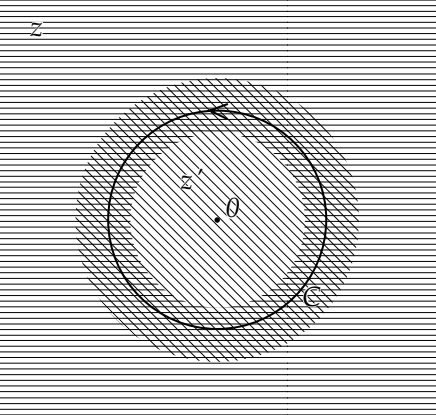
\includegraphics[width=0.5\textwidth]{figure/Fig5.3.jpg}\\
		\caption{Coordinate patches $z^{\prime}$ (diagonal hatching) and $z$ (horizontal hatching) with vertex operator at $z^{\prime}=0$. In the annular region, $z=z^{\prime}+z_{v}$.}\label{Fig5.3}
	\end{center}
\end{figure}

We keep the vertex operator at $z^{\prime}=0$ and encode its position into the transition function:
\begin{equation}
	z=z^{\prime}+z_{v}\label{5.4.16}
\end{equation}
The measure for $z_{v}, \bar{z}_{v}$ is given by \eqref{5.4.15}, where:
\begin{equation}
	\left.\frac{\partial z^{\prime}}{\partial z_{v}}\right|_{z}=-1\label{5.4.17}
\end{equation}
Therefore, the ghost insertion is:
\begin{equation}
	\int_{C} \frac{d z^{\prime}}{2 \pi i} b_{z^{\prime} z^{\prime}} \int_{C} \frac{d \bar{z}_{m}^{\prime}}{-2 \pi i} b_{\bar{z}^{\prime} \bar{z}^{\prime}}=b_{-1} \tilde{b}_{-1}\label{5.4.18}
\end{equation}
where $C$ is any contour surrounding the vertex operator as shown. Then, the complete expression for the $S$-matrix can be compactly written as:
\begin{equation}
	S(1 ; \ldots ; n)=\sum_{\text {compact topologies}} e^{-\lambda \chi} \int_{F} \frac{d^{m} t}{n_{R}}\left\langle\prod_{k=1}^{m} B_{k} \prod_{i=1}^{n} \hat{\mathscr{V}}_{i}\right\rangle\label{5.4.19}
\end{equation}
Here, $B_{k}$ is shorthand for the $b$ ghost insertion \eqref{5.4.15}, and $\hat{\mathscr{V}}$ represents $\tilde{c} c \mathscr{V}_{\mathrm{m}}$ for closed strings and $t_{a} c^{a} \mathscr{V}_{\mathrm{m}}$ for open strings. That is, we now treat all vertex operators as fixed and replace their coordinates with extra parameters in the transition functions. The number of moduli $m$ is:
\begin{equation}
	m=\mu+2 n_{\mathrm{c}}+n_{\mathrm{o}}-\kappa=-3 \chi+2 n_{\mathrm{c}}+n_{\mathrm{o}}
\end{equation}
where $n_{\mathrm{c}}$ and $n_{\mathrm{o}}$ are the numbers of closed string and open string vertex operators, respectively.

\eqref{5.4.19} shows that hatted vertex operators, i.e., those containing $\tilde{c} c$ or $t_{a} c^{a}$, are fundamental. This is exactly what the state-operator correspondence produces, and it is BRST-invariant. If the vertex operator is integrated, the ghost insertion \eqref{5.4.18} will remove $\tilde{c} c$ or $t_{a} c^{a}$. For example:
\begin{equation}
	b_{-1} \tilde{b}_{-1} \cdot \tilde{c} c \mathscr{V}_{\mathrm{m}}=\mathscr{V}_{\mathrm{m}}
\end{equation}
leaving the integrated form of the vertex operator. We wrote \eqref{5.4.19} from the Polyakov path integral, so vertex operators appear in the form of OCQ, but now we can use any BRST-invariant vertex operator.